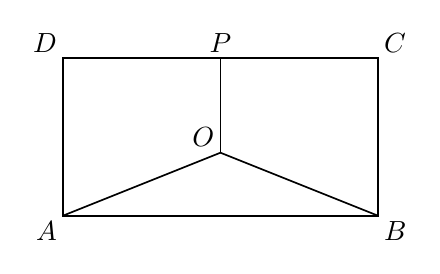
\begin{tikzpicture}[x=1cm,y=1cm,font=\normalsize,
 geometry edge/.style={solid,line width=.6pt},
 geometry mark/.style={solid,line width=.6pt},
 geometry label/.style={font=\normalsize,inner sep=2pt}]
\coordinate (A) at (0.0,0.0);
\coordinate (B) at (4.0,0.0);
\coordinate (C) at (4.0,2.0);
\coordinate (D) at (0.0,2.0);
\coordinate (P) at (2.0,2.0);
\coordinate (O) at (2.0,0.8);
\draw[geometry edge] (A)--(B)--(C)--(D)--cycle;
\draw[geometry edge] (P)--(O);
\draw[geometry edge] (A)--(O);
\draw[geometry edge] (B)--(O);
\node[geometry label,below left] at (A) {$A$};
\node[geometry label,below right] at (B) {$B$};
\node[geometry label,above right] at (C) {$C$};
\node[geometry label,above left] at (D) {$D$};
\node[geometry label,above] at (P) {$P$};
\node[geometry label,above left] at (O) {$O$};
\end{tikzpicture}